% TeX program = xelatex
\documentclass{ctexart}
\usepackage{graphicx}
\usepackage{geometry}
\usepackage{amsfonts,amssymb,amsthm,amsmath,physics,extarrows}
\usepackage{mathrsfs}
\usepackage{tikz}
\usepackage{hyperref}% 这样可以有超链接(可以点击翻页)
\usepackage{simpler-wick}% wick收缩
\usepackage{arydshln}% 虚线

\usetikzlibrary{arrows.meta,decorations.markings,calc,bending}



\newtheorem{definition}{定义}[section]
\newtheorem{lemma}{引理}[section]
\newtheorem{theorem}{定理}[section]
\newtheorem{proposition}{命题}[section]
\newtheorem{example}{例}[section]

\newcommand{\bm}[1]{\boldsymbol{#1}}
%这行是用来支持latex-workshop预览的

\numberwithin{equation}{section}
	% 请检查相对路径是否有效
\title{场论与凝聚态笔记}
\author{mny}

\usepackage{caption} % 自定图片标题
\captionsetup[figure]{name=Fig, labelsep=period}
\numberwithin{figure}{section}

\usepackage{wrapfig} % 图片文字混排
\begin{document}

\maketitle
\tableofcontents

% !TeX root = 场论与凝聚态.tex
\section{Invitation: The Cartoon of Confinement}
Never see individual quarks.

For separatable particles, like electron charges, their potential is 
$V(r) \sim \frac{1}{r}$, thus $V(r)-V(r_0)$ is always bounded.

Two quarks forms a pion. They interacts through gluon, and forms a structure called gluon tube or string. The potential is $V(r) \sim r$ and the energy density per length is appropriately constant. To separate a quark pair, the energy inputed $V(r)-V(r_0)$ is unbounded.

Similar phenomenon appears in superconductor(type II). When electronic charge condensed, the interaction of magneticmonopole becomes $V(r) \sim r$. According to EM duality, when magneticmonopole condensed, analogy goes to its counterpart. (Perspective by t'Hooft, Polyakov and Manldstan.)

\section{Path Integral for Single Particles}
From the two-slit interference, we've known the picture of wave. Whilst, the view of particle could recover the result by computing the phase $\mathrm{e}^{\mathrm{i} S}$.

For single particle mechanic, we start from the Schr\"odinger equation
\begin{equation}
  \mathrm{i} \hbar \partial_t \ket{\psi(t)} = H(p,x,t) \ket{\psi(t)}.
\end{equation}
We have the time evolution operator
\begin{equation}
  \ket{\psi(t)}=U(t,t_0)\ket{\psi(t)},
\end{equation}
which is unitary,
\begin{equation}
  U^{\dagger}(t,t_0) U(t,t_0) = 1.
\end{equation}

If $H$ is time-dependent, we split the time interval into small slices, and we get the infinitesimal $U$ operator as time-independent cases,
\begin{equation}
  U(t,t_0) = \prod_{n=0}^{N-1} U(\overbrace{t_{n-1}, t_{n}}^{\delta t}),
\end{equation}
where $t_n \equiv t + n \delta t$. Note that the product is time ordered.

Another perspective is from the Schr\"odinger equation, by finite differential,
\begin{equation}
  \ket{\psi(t+\delta t)} = \left[ 1- \frac{\mathrm{i} }{\hbar}H(p, x, t+ \frac{\delta t}{2}) \right] \ket{\psi(t)}
\end{equation}
To the order of $\delta t$, we have 
\begin{equation}
    \ket{\psi(t+\delta t)} = \mathrm{e}^{- \frac{\mathrm{i} }{\hbar}H(p,x,t+ \frac{\delta t}{2})} \ket{\psi(t)}
\end{equation}

Next, we put the time evolution operator in spacial basis, considering
\begin{equation}
  \bra{x'}U(t+\delta t,t)\ket{x}.
\end{equation}
Suppose $H = \frac{p^{2}}{2m}+ V(x)$ for simplicity, we obtain
\begin{equation}
  \bra{x'}\left[ 1- \frac{\mathrm{i}  \delta t}{\hbar}\left( \frac{p^{2}}{2m} + V(x, t+ \frac{\delta t}{2}) \right)  \right] \ket{x}.
\end{equation}
Make a substitution
\begin{equation}
  V \rightarrow \frac{V(x',t+ \frac{\delta t}{2})+ V(x, t+\frac{\delta t}{2})}{2} 1,
\end{equation}
and insert a completeness relation of $p$ in each time slice, we arrive at
\begin{equation}
    \bra{x'}U(t+\delta t,t)\ket{x} = \int_{}^{} \mathrm{d}p \, \frac{1}{2\pi\hbar} \mathrm{e}^{\frac{\mathrm{i} p(x'-x)}{\hbar}} \exp \left[ - \frac{i\delta t}{\hbar} \frac{H(p,x',t+ \frac{\delta t}{2})+H(p,x,t+ \frac{\delta t}{2})}{2} \right] .
\end{equation}
written in a more compact form,
\begin{equation}
    \bra{x'}U(t+\delta t,t)\ket{x} \sim \int_{}^{} \mathrm{d}p \, \frac{1}{2\pi\hbar} \mathrm{e}^{\mathrm{i} \frac{p \delta x}{\hbar}-\mathrm{i}  \frac{H \delta t}{\hbar}}. 
\end{equation}

The finite-time evolution operator,
\begin{equation}
  U(t_N, t_0) = \prod_{n=0}^{N-1} U(t_{n-1},t_n)
\end{equation}
inserting an identity operator as $x$ basis completeness relation,
the element is 
\begin{equation}
  U(t_{n+2},t_{n+1}) \underbrace{{1}}_{\int_{}^{} \mathrm{d}x_n \, \ket{x_n}\bra{x_n} } U(t_{n+1},t_{n})
\end{equation}
then we obtain
\begin{equation}
  \begin{aligned}
    \bra{x_N}U(t_N, t_0)\ket{x_0}
    & = \left( \prod_{n=1}^{N-1} \int_{}^{} \mathrm{d}x_n \, \bra{x_{n+1}}U(t_{n+1},t_{n}) \ket{x_n}  \right) 
    \\
    & \times \bra{x_1}U(t_1,t_0)\ket{x_0}
    \end{aligned}  
\end{equation}
in full,
\begin{equation}
  \begin{gathered}
    \bra{x_N}U(t_N, t_0)\ket{x_0}
    =\left( \prod_{n=1}^{N-1} \int \frac{\mathrm{d} p_{n+ \frac{1}{2}} \, \mathrm{d} x_n}{2\pi \hbar} \right) \int \frac{\mathrm{d} p_{\frac{1}{2}}}{2\pi \hbar} 
    \\
    \times \exp \left( \frac{\mathrm{i} }{\hbar} \sum_{n=0}^{N-1} \left[ p_{n+ \frac{1}{2}}(x_{n+1}-x_n) - \delta t  \frac{H(p_{n+ \frac{1}{2}},x_{n+1}, t_{n+ \frac{1}{2}})+H(p_{n+ \frac{1}{2}},x_{n}, t_{n+ \frac{1}{2}}) }{2}\right]  \right) 
    \\
    \sim \left( \prod_{n=0}^{N-1} \int \frac{\mathrm{d} p_{n+ \frac{1}{2}} \, \mathrm{d} x_n}{2\pi \hbar} \right) \int \frac{\mathrm{d} p_{\frac{1}{2}}}{2\pi \hbar} \mathrm{e}^{\frac{\mathrm{i} }{\hbar} \int p\, \mathrm{d} x - H \, \mathrm{d} t}
  \end{gathered}
\end{equation}
% !TeX root = 场论与凝聚态.tex


Insert a operator $\hat{B}(x)$ in between the path integral, 
\begin{equation}
    \begin{gathered}
        \bra{x_N} U(t_N, t_m) \hat{B}(x) U(t_m, t_0) \ket{x_0} = 
        \left( \prod_{n=1}^{N-1} \int \frac{\mathrm{d} p_{n+\frac{1}{2}}\mathrm{d} x_n}{2\pi \hbar} \right) \int \frac{\mathrm{d} p_{\frac{1}{2}}}{2\pi\hbar} 
        B(x_m)
        \\
        \times \exp \frac{\mathrm{i} }{\hbar} \sum_{n=0}^{N-1} \left[ p_{\frac{1}{2}}(x_{n-1}- x_{n})  - \delta t \frac{H(p_{n+\frac{1}{2}}, x_{n+1}, t_{n+\frac{1}{2}}) + H(p_{n+\frac{1}{2}}, x_{n}, t_{n+ \frac{1}{2}})}{2}\right] .
    \end{gathered}
\end{equation}
We simply need to add the value of the operator as a function of certain space coordinate in the expression of path integral.

\section{Observables in QM}
\begin{itemize}
  \item \begin{equation}
    \bra{\psi} A \ket{\psi}, \ A^{\dagger} = A.
  \end{equation}

  \item Probability of projection,
  \begin{equation}
    P = |\bra{\phi}\ket{\psi}|^2 = \bra{\psi} \underbrace{\ket{\phi} \bra{\phi}}_{\hat{A}}\ket{\psi}
  \end{equation}
  
  \item Observables after evaluation,
  \begin{equation}
    \bra{\phi} \underbrace{\mathrm{e}^{\mathrm{i} H t / \hbar} A \mathrm{e}^{- i H t / \hbar}}_{\hat{A}(t)} \ket{\psi}
  \end{equation}

  \item Projection after evaluation: scattering
  \begin{equation}
    P = |\bra{\psi} \mathrm{e}^{- \mathrm{i}  Ht / \hbar}\ket{\psi}|^2 = \bra{\psi} \underbrace{\mathrm{e}^{\mathrm{i} H t / \hbar} \ket{\phi}\bra{\phi} \mathrm{e}^{- i H t / \hbar}}_{\hat{A}(t)} \ket{\psi}
  \end{equation}

  \item Retarded correlation
  \begin{equation}
  H(t) = H_0 + \underbrace{a(t)}_{\text{small}} B.
\end{equation}
  The contribution of $\bra{\psi}U^{\dagger}(t,0) A U(t,0)\ket{\psi}$ to the first order correction in $a$ is
  \begin{equation}
    - \frac{\mathrm{i} }{\hbar} \int \mathrm{d} t' a(t')\Big[ \bra{\psi}U_0^{\dagger}(t,0) A U_0(t,t') B U_0(t',0) - U_0^{\dagger}(t,0) B U_0(t,t') A U_0(t',0)\ket{\psi} \Big] 
  \end{equation}



\end{itemize}



\section{Path Integrals for Fields}
There's a mattress with springs and massive balls connected. Denoting the offset of each ball as $\phi_{\vec{r}}$ the Hamiltonian is
\begin{equation}
  H = \sum_{\vec{r} \text{ on lattice}}\left[ \frac{p_{\vec{r}}^2}{2m} + V(\phi_{\vec{r}}) + \sum_{\hat{\tau} = 1}^d \frac{k}{2}\left( \phi_{\vec{r} + \alpha \vec{\tau}}  - \phi_{\vec{\tau}}\right)^2  \right] ,
\end{equation}
with a commutation relation 
\begin{equation}
  \left[ \phi_{\vec{r}}, p_{\vec{r}'} \right]  = \mathrm{i}  \hbar \delta_{\vec{r},\vec{r}'}.
\end{equation}
The interacting part of the Hamiltonian only involves pairs nearby.

In continuum limit, $\displaystyle H = \int \mathrm{d} ^{d}\vec{r} \mathcal{H}(\vec{r})$, and we can write the Hamilton density as
\begin{equation}
  \mathcal{H}  = \frac{\pi(\vec{r})^2}{2\rho} + \mathcal{V} (\phi(\vec{r})) + \frac{\kappa}{2} \left[ \partial_{\vec{r}} \phi(\vec{r}) \right] ^2,
\end{equation}
where $\displaystyle \pi(\vec{r}) = \frac{p_{\vec{r}}}{\alpha^d}, \mathcal{V} = \frac{V}{\alpha^d}, \rho = \frac{m}{\alpha^d}, \kappa = \frac{k\alpha^2}{\alpha^d}$.

\paragraph{Path Integral}
At $t_n$, we use $\bigotimes_{\vec{r}} \ket{\phi(\vec{r})} $ basis, and $\bigotimes_{\vec{r}} \ket{\pi(\vec{r})} $ for $t_{n + \frac{1}{2}}$. 

Analogously, we get
\begin{equation}
    \begin{gathered}
        \bra{\text{end}}U(t,0)\ket{\text{start}} = 
        \left( \prod_{t_n, \vec{r}} \frac{\mathrm{d} p_{t_n+\frac{1}{2}, \vec{r}} \ \mathrm{d} \phi_{t_n, \vec{r}}}{2\pi\hbar}  \right) _{\text{suitable boundary condition}}
        \\
        \times \exp
        \frac{\mathrm{i} }{\hbar} \sum_{t_n, \vec{r}}\left[ 
            p _{t_{n+\frac{1}{2}}, \vec{r}}\left( \phi_{t_{n+1}, \vec{r}} - \phi_{t_n, \vec{r}} \right)
            -\delta t \left( 
                \frac{p_{n+ \frac{1}{2}, \vec{r}}^2}{2m} + \frac{k}{2} \sum_{\hat{\tau} = 1}^d \left( \phi_{t_{n}, \vec{r} + \alpha \hat{\tau} } - \phi_{t_n, \vec{r}} \right) ^2 + V(\phi_{t_n, \vec{r}})
             \right)  
         \right] .
    \end{gathered}
\end{equation}
Integrate out $p$, we obtain
\begin{equation}
  \begin{gathered}
    \left( \prod_{t_n, \vec{r}} \sqrt{\frac{2\pi\hbar m}{\mathrm{i} \delta t}} \frac{\mathrm{d} \phi_{t_n, \vec{r}}}{2\pi\hbar}  \right) _{\text{suitable boundary condition}}
    \\
    \times 
    \exp \frac{i\delta}{\hbar} \sum_{t_n, \vec{r}} 
     \left[  
            \frac{m}{2}\left( \frac{\phi_{t_{n+1},\vec{r}} - \phi_{t_n, \vec{r}}}{\delta t} \right)  - \frac{k\alpha^2}{2} \sum_{\hat{\tau} = 1}^d \left( \frac{\phi_{t_{n}, \vec{r} + \alpha \hat{\tau} } - \phi_{t_n, \vec{r}}}{\alpha} \right) ^2 - V(\phi_{t_n, \vec{r}})
     \right],
  \end{gathered}
\end{equation}
in which time and space stand in the same place, similar to relativistic K-G field.


\section{Free Field Theory}
For free fields, $V(\phi_{\vec{r}}) = \frac{u}{2}\phi_{\vec{r}}^2$, it behaves just like coupled simple harmonic oscillators.
To find the normal modes, we use Fourier transformation.
\begin{equation}
  \phi_{\vec{r}} = \int_{-\frac{\pi}{\alpha}}^{\frac{\pi}{\alpha}} \frac{\mathrm{d}^d \vec{k}}{(2\pi)^d} \, \mathrm{e}^{\mathrm{i} \vec{k}\cdot \vec{r}}\phi_{\vec{k}} ,
\end{equation}
likewise for $p_{\vec{r}}$.

$\phi_{\vec{r}}$ is real, thus $\phi_{\vec{r}} = \phi_{\vec{r}}^\dagger \implies \phi_{-\vec{k}} = \phi_{\vec{k}}^\dagger$, and the commutation relation is
\begin{equation}
  \left[ \phi_{\vec{k}}, p_{\vec{k}'} \right] = \mathrm{i} \hbar (2\pi)^d \delta^{d}(\vec{k} + \vec{k}').
\end{equation}

The Hamiltonian becomes
\begin{equation}
  H = \int_{-\frac{\pi}{\alpha}}^{\frac{\pi}{\alpha}} \frac{\mathrm{d} ^d \vec{k}}{(2\pi)^d}\frac{1}{2}
  \left[ 
    \frac{p_{-\vec{k}}p_{\vec{k}}}{2m} + \left( \frac{k}{2} \sum_{\vec{\tau} = 1}^d \left( 2 \sin \frac{\alpha k_i}{2} \right) ^2 + \frac{u}{2}  \right) \phi_{-\vec{k}}\phi_{\vec{k}}
   \right] ,
\end{equation}
from which we can directly figure out the frequency $\omega_{\vec{k}} = \omega_{-\vec{k}} = \sqrt{\frac{k \sum_{\vec{\tau}} \left( \sin \frac{\alpha k_i}{2} \right) ^2 + U}{m}}$

Next, we need to make a substitution, or Bogoliubov transformation:
\begin{align}
  \phi_{\vec{k}}^c = \frac{\phi_{\vec{k}}+\phi_{-\vec{k}}}{\sqrt{2}},
  \\
  \phi_{\vec{k}}^s = \mathrm{i} \frac{\phi_{\vec{k}} - \phi_{-\vec{k}}}{\sqrt{2}}.
\end{align}
the integration range becomes half of $\vec{k}$.




\subsection{Ground State Wave Function and Entanglement}

\subsection{Energy Gap and Correlation}
There's no gapless excitations in finite crystal constant lattice theory since the minimal wave number is $\sim  \frac{\pi}{a}$
% !TeX root = 场论与凝聚态.tex

\section[The Origin of $\mathrm{i} 0^{+}$]{Where comes the $ \mathrm{i} 0^{+}$: a Non-Perturbative Interpretation}
Unitarity and locality plays an unreplaceable role in QFT and a lot of deep conclusion can be gained directly from these two properties, without the need of calculation of specific model.

In QFT, we compute something like
\begin{equation}
  \bra{\phi} \cdots \ket{\psi}, \ \text{or}\ \int_{\text{b.c.}} \mathcal{D} (\square)  \exp \left( \cdots \right) ,
\end{equation}
respectively in operator and path integral methodology, and b.c. stands for boundary condition.

In condensed matter, the experiment are done by disturbing a ground state, and the system would decay from excited state to ground state eventually, thus (near $T \sim 0$) what we usually compute is
\begin{equation}
   \bra{0} \cdots \ket{0}.
\end{equation}
And in particle phys., after performing LSZ reduction, any initial or final state would be turned into creation/annihilation operators acting on a ground state, thus, similarly, we compute
\begin{equation}
  \bra{\phi}\cdots \ket{\psi} \to  \bra{0} O^{\dagger}_{\phi} \cdots O_{\psi}\ket{0}.
\end{equation}

Furthermore, it seems that we need to get the wave function of ground state ,which would be extremely hard in any theory with interaction, however, we do not actually need to do so. The following of this section would explain it in detail.

A typically computation would be in the form of
\begin{equation}
  \bra{\phi} \mathrm{e}^{ \mathrm{i} t_f H} \mathrm{e}^{\mathrm{i}  t_i H} \ket{\psi},
\end{equation}
where the initial and final time are set at $-\infty$ and $+\infty$ for the reason that the time interval of a physical process would be greatly smaller that of an experiment.

\paragraph{Operator}
A commonly used trick is to make a substitution of $\mathrm{e}^{- \mathrm{i} \Delta t H} \to \mathrm{e}^{- i\Delta t H \left( 1- \mathrm{i}  0^{+} \right) }$ in time evolution. \footnote{It is no longer unitary, but that's what we want.}
Let's check its property in two cases: finite time and infinite time.
When $\Delta t$ is finite, there's nothing abnormal. When $\Delta t \to  + \infty$, a factor of exponentially suppress appears, yet except for states whose $H = 0$. This term would effectively become $\ket{0} \bra{0}$ or $\sum_i \ket{0_{i}} \bra{0_{i}}$ when $H \ket{0} = 0$.

If, unfortunately, the experiment time isn't literally infinite, the $0^{+}$ have to be
\begin{equation}
  0^{+} \sim \frac{1}{\text{experiment time}}\quad (\text{or relaxation time } t).
\end{equation}

In Green function, this projection to ground state is included by substitution of
\begin{equation}
   \begin{aligned}
     \omega \to \left( 1 + \mathrm{i} 0^{+} \right) \omega \quad &\text{(time ordered)}
     \\
     \omega \to \omega + \mathrm{i}  0^{+}\quad &\text{(retarded)}
   \end{aligned}.
\end{equation}

\paragraph{Path Integral}
After a substitution of $H \delta t \to H \left( 1-\mathrm{i}  0^{+} \right) \delta t$, we obtain
\begin{equation}
  \int_{\text{No b.c.}} \mathcal{D} p \, \mathcal{D} x \, \exp \left( \frac{\mathrm{i} }{\hbar} \int \left[ p\, \mathrm{d} x - H \left( 1-\mathrm{i} 0^{+} \right) \, \mathrm{d} t\right]  \right) .
\end{equation}

\paragraph{Wick Rotation}
In the process given above, we have \emph{rotated} the trajectory of $t$ from the real axis to another line through the original point with a small angle $0^{+}$. A generalization of this trick is to choose a integral contour along the imaginary axis, which is called \emph{Wick rotation}. 
It can be shown that, in principle, if we know all observables along the $z = -\mathrm{i} \tau$ axis, all observables on real time can be recovered to the spirit of analytical continuation.
\begin{figure}[h]
  \centering
  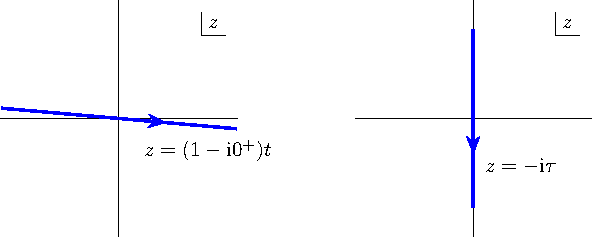
\includegraphics{figures/wick_rotation.pdf}
  \caption{Wick rotation}
\end{figure}
Under this, the expression of path integral becomes 
\begin{equation}
  \int \mathcal{D} \pi \, \mathcal{D} \phi \, \exp \left[ \frac{\mathrm{i} }{\hbar} \int \mathrm{d} \tau \, \mathrm{d} ^{3} r \left( \pi \mathrm{i}  \partial_{t} \phi - \mathcal{H} \right)  \right] .
\end{equation}
This formalism is also called \emph{Euclidean field theory} or \emph{imaginary time} path integral.

The name ``Euclidean'' field theory comes from the fact that after completing the integration on $\pi$ of a free field, we would find the term on the exponential becomes
\begin{equation}
  \mathcal{L}_{\text{Euclidean}}\sim \left( \partial_{t} \phi \right) ^{2} + \left( \partial_{\vec{r}} \phi \right) ^{2} + \phi^{2},
\end{equation}
instead of the Lagrangian density in Minkovski spacetime, whose form is typically 
\begin{equation}
  \mathcal{L}_{\text{Minkovski}} = \left( \partial\phi \right) ^{2} - m^{2} \phi^{2} = \left( \partial_{t} \phi \right) ^{2} - \left( \partial_{\vec{r}} \phi \right) ^{2} - m^{2} \phi^{2}.
\end{equation}
The iconic minus signs from Minkovski metric were eliminated after Wick rotation as if it morphed into a field living in Euclidean space.


\section{Dualities of QFT and Stat. Mech.}
\subsection{Partition Function as Path Integral}
In statistic mechanics, we compute the partition functions of fields,
\begin{equation}
  \mathcal{Z} = \sum_{s} \mathrm{e}^{-\beta E_{s}} = \sum_{s} \mathrm{e}^{-\beta \int \mathrm{d} \vec{r} \, \mathcal{H}},
\end{equation}
which is easy to compute in classical statistic mechanics where $\hbar = 0$, i.e., all operators commute.

However, in quantum cases, the calculation of
\begin{equation}
  \mathcal{Z} = \Tr \left( \mathrm{e}^{- \beta H} \right) = \Tr \left( \mathrm{e}^{-\beta \int \mathrm{d}^{d} \vec{r} \, \mathcal{H} } \right) 
\end{equation}
becomes impossible, because energy eigenstates are non-local and the eigenvalues of Hamiltonian are hard to find.
To solve this, we consider the $\mathrm{e}^{-\beta H}$ as a product of a series of $\mathrm{e}^{-\beta \epsilon}$. By analogy, we insert a completeness relation of momenta and field operators in between each of them. Whereby, we get
\begin{equation}
  \mathcal{Z} = \prod_{\vec{r}, t}^{} \left( \frac{1}{2\pi\hbar} \int \mathrm{d} \pi_{\tau + \frac{\delta \tau}{2}, \vec{r}} \, \mathrm{d} \phi_{\tau, \vec{r}}  
  \right)  
  \exp \left[ \frac{1}{\hbar} \int_{0}^{\beta\hbar} \mathrm{d}\tau \,\mathrm{d} ^{d} r\, \left( \pi \mathrm{i}  \partial_{\tau} \phi - \mathcal{H}\left( \pi, \phi \right)  \right) \right] 
\end{equation}
This expression is local
\footnote{
  It is of full necessity to indicate that a theory with locality means it is defined locally and does not have to live in $\mathbb{R}^{d} \times \mathbb{S}^{1}$ (or $\mathbb{R}^{d} \times  \mathbb{R}^{1}$).
}
in space``time'', with the cost of introducing an additional dimension on $\mathbb{S}^{1}$ (note that calculating trace implies that initial state and final state are the same thus this dimension is rolled up.) \textbf{We have clearly verified that a $d$-dim space statistic field theory is close related to a QFT in $(d+1)$-dim spacetime.}

\begin{itemize}
  \item When $\beta \to \infty$, it becomes the Euclidean QFT.
  \item When $\hbar \to  0$,
  \begin{equation}
    \frac{1}{\hbar} \int^{\hbar \beta} \mathrm{d} \tau \, \left( \square \right) \to \beta \frac{\partial }{\partial \tau} \int \mathrm{d} \tau \, \left( \square \right)  \to  \beta \left( \square \right) ,
  \end{equation}
  hence it goes back to classical case.
\end{itemize}

Additional compatibilities can be intuited directly from the form of path integral mopped up the momentum $\pi$, listed as follows:
\begin{equation*}
  \begin{matrix}
      d\text{-space quantum Stat. Mech.}\\
      \Updownarrow \\
      (d+1) \text{-spacetime QFT}\\
      \Updownarrow \\
      (d+1) \text{-space classical Stat. Mech.}
  \end{matrix}
\end{equation*}

The statistic field theory integrated out momenta is
\begin{equation}
  \mathcal{Z} = \int \mathcal{D} \phi  \, \exp\left[ - \int \underbrace{\mathrm{d} \tau \, \mathrm{d} ^{d} r}_{\mathrm{d} ^{d+1} r \text{ in } \Sigma \times \mathbb{S}^{1}}\, \left( \frac{\left( \partial_{\tau} \phi \right) ^{2}}{2} + \frac{\left( \partial_{\vec{r}} \phi \right) ^{2}}{2} + V\left( \phi \right)  \right) \right] 
\end{equation} 
which can be rewritten as
\begin{equation}
  \mathcal{Z} = \int \mathcal{D} \phi \, \exp \left[ - \int \mathrm{d} ^{d+1} r \, \left( \frac{\left( \partial_{\tau} \phi \right) ^{2}}{2} + \frac{\left( \partial_{\vec{r}} \phi \right) ^{2}}{2} + V\left( \phi \right)  \right)  \right] .
\end{equation}
It can be reinterpreted as classical stat. mech. in $(d+1)$-space, whose, however, $\tilde{\beta}$ has no physical reflections.


% !TeX root = 场论与凝聚态.tex
There might be a puzzle through the derivation above, 
\begin{quote}
    \emph{Before integrating out $\pi$, the $\exp$ term contains $\pi \mathrm{i} \partial_{\tau} \phi$. This match seems presentation-depending.
    How to figure out this mapping in a presentation independent way?}
\end{quote}


\subsection{General Development}
We' ve seen that a quantum field theory in $d+1$-dim spacetime can be reinterpreted as a $d$-dim space statistic field theory by regarding the time dimension as a inverse temperature, but it is not so obvious when we did not mop up the integration of conjugate momenta $\pi$. We need to find a way in whole, to figure out in what situation a quantum field theory can be seen as a statistic field theory. \emph{``Just as the time when we heard about the formalism of Lagrangian mechanic, all cumbersome processes of force analysis disappeared.''}

\textbf{The answer is by locality and unitarity.}

Let us first compare the behaviors between QFT and stat. mech.
\footnote{
    The properties mentioned in the table are only valid with an implicit assumption that the base manifold of the field is orientable.
}
\begin{center}
    \begin{tabular}{|c|c|}
        \hline
        Real time & Imaginary time\\ 
        \hline & \\
        unitarity & reflection positivity\\ & \\
        \hline & \\
        \parbox{5cm}{\centering
            $\left( \mathrm{e}^{- \mathrm{i} H \Delta t} \right)^{*} = \mathrm{e}^{ - \mathrm{i} H (- \Delta t) }$
            \\
            $\Downarrow$
            \\
            $\mathop{\mathcal{Z}_{\mathbb{R} \times \Sigma}^{*} = \mathcal{Z}_{\mathop{\bar{\mathbb{R}}}\limits^{}_{\uparrow} \times \Sigma}}\limits^{}_{
                \hspace{5em} \text{orientation inversed}
                }
            $
            }&
        
        \parbox{5cm}{\centering
            also true because the only imaginary part is $\mathrm{e}^{- \int \mathrm{d} \tau \, \pi \mathrm{i}  \partial\tau \phi}$
            \\
            $\implies \mathcal{Z}^{*}_{\Sigma'} = \mathcal{Z}_{\bar{\Sigma}'}$
        } \\ & 

        \\ \hline

        \multicolumn{2}{|c|}{}\\

        \multicolumn{2}{|c|}{
            \parbox[h]{15cm}{The partition function of a locally defined theory can be splited into two parts, each on half of the base manifold. 
            For $\Sigma = \parbox{2.8cm}{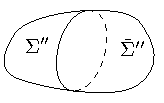
\includegraphics{figures/orientable_base.pdf}}$,
            the degree of freedom is the arbitrary boundary condition on $\partial \Sigma''$.
            By treating $\mathcal{Z}_{\Sigma''}$ and $\mathcal{Z}_{\bar{\Sigma}''}$ as functionals of $\left. \phi \right|_{\partial \Sigma''}$.
            we have 
            $$
            \mathcal{Z}_{\Sigma'} = \int  \left.\mathcal{D} \phi \right|_{\partial \Sigma''} \mathcal{Z}_{\Sigma''} \mathcal{Z}_{\bar{\Sigma}''} = \int  \left.\mathcal{D} \phi \right|_{\partial \Sigma''} \left( \mathcal{Z}_{\Sigma''} \right)  ^{2} \ge  0
            $$
            } 
        }\\
        \multicolumn{2}{|c|}{}\\
        \hline & \\

        \parbox{6cm}{\centering
            time reversal invariant \\
            $\Downarrow$ \\
            $\begin{cases} 
                \mathcal{Z}_{\Sigma' \times \bar{\mathbb{R}}} = \mathcal{Z}_{\Sigma' \times \mathbb{R}} \\
                \mathcal{Z}_{\Sigma'}^{*} = \mathcal{Z}_{\bar{\Sigma}'}
              \end{cases}
            $\\
            $\Downarrow$ \\
            $\mathcal{Z}$ is always real.
            }&
        \parbox{6cm}{
            \centering also \\ (useful in \emph{topological insulator})
            }
            \\ & \\
            \hline
        
    \end{tabular}
\end{center}
\clearpage
We have came to the conclusion that a theory with locality (of course with Hermitian Hamiltonian whilst) is always accompanied by a real and positive partition function $\mathcal{Z}$.



In the following it will be convinced that \emph{if and only if} the generative functional of a Euclidean field theory is real and positive, it has a \emph{classical stat. mech. interpretation}.

Sufficiency can be easily verified, as we have
\begin{equation}
  \mathcal{Z} = \int \mathcal{D} \phi  \, \exp\left( - \beta \int \mathrm{d} ^{d+1} r' \, \mathcal{H}(\phi) \right),
\end{equation}
no imaginary part appears in the expression of $\mathcal{Z}$.
\footnote{The integration of $\mathcal{D} \phi $ can be approximated by summation on a large amount of field configurations, which turns out to be Mont Carlo method for stat. mech.}

Proof of necessity is carried out by utilizing locality, as path integral can be performed in a certain subset on spacetime.\footnote{but there's no locality in momentum space.}
\begin{figure}
    \centering
    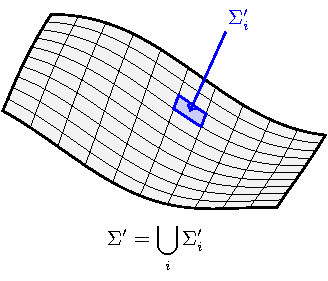
\includegraphics{figures/splited_base_manifold.pdf}
    \caption{Splited base manifold}
    \label{split_manifold}
\end{figure}
Splitting the base manifold into small parts, as shown in Fig\ref{split_manifold}, the path integral on each sub-manifold is fully determined by the b.c. on each $\partial\Sigma'_{i}$. Hence the path integral on $\Sigma'$ can be expressed as
\begin{equation}
    \mathcal{Z}_{\Sigma'} = \int \left( \text{b.c. of all boundary} \right) \prod_{i} \mathcal{Z}_{\Sigma' _{i} \text{ (b.c.)}}.
\end{equation}
Given that locality and unitarity guarantee that all $\mathcal{Z}_{\Sigma'_{i}}$ are \emph{real and positive}, such $\mathcal{Z}_{\Sigma'_{i}}$ is undoubtedly doable to be turned into the form of $\mathrm{e}^{- \tilde{\beta} \left( \cdots \right) }$, thus there always exists an effective Hamiltonian density and corresponding inverse temperature to match this QFT with a stat.~mech. interpretation.


\section[When do Symmetries Break Spontaneously]{SSB: What is Broken? Why no Tunneling?}

A name of ambiguity was designated to refer as the physical picture behind SSB, resulting a widespread misconstruction among juvenile learners, that ``\emph{a potential with minimal value at non-zero field strength will lead to SSB as vacuum state is static and tends to minimize its Hamiltonian.}'' But such explanation will be no longer compatible if one try to replicate this in a statistic field theory and he would eventually figure out that the ensemble expectation value of field strength in ground state will remain zero. 

To answer the question of what is breaking, we need to investigate a simplest case, that is, a $0$-dim field. 
\begin{figure}[hp]
    \centering
    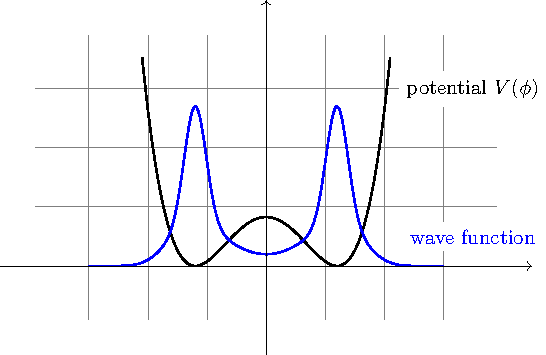
\includegraphics{figures/double_minimum_potential.pdf}
    \caption{$1$-dim field in a double-minimal potential}
    \label{1d_double_minimal}
\end{figure}
The picture of a $0$-dim field is generally characterized by Fig\ref{1d_double_minimal}. Directly from the figure, one can discover that the vacuum expectation value of $\phi$ is $0$, even though the field is trapped in a potential with two valleys. The key is that as long as the shape of potential is not so sharp, a non-zero tunneling amplitude will gradually expunge any symmetry-broken state as time evolutes. We need to get a approach to form a \emph{naturally} infinite potential barrier, i.e. at least one parameter of the system should go to infinite under some limit.

In a system with infinite degrees of freedom, we describe it by a Hamiltonian density, thus
\begin{equation}
    V\left( \phi=0 \right) \propto \text{ volume of space}.
\end{equation}
Hence, a spontaneous symmetry broken only appears under thermodynamic limit.

In the following we need to develop a well-defined language of SSB, since the ambiguity of describing SSB as a shifted vacuum expectation field strength will keep bothering us as long as we are motivated to investigate phenomena of SSB in stat. mech.
A double-minimum potential would lead to degeneracy of ground state. To avoid this, we introduce a background magnetic field $B$, the free energy will be modified to
\begin{equation}
  F = \tilde{F} - B \tilde{M} \cdot \text{Vol}.
\end{equation}
% !TeX root = 场论与凝聚态.tex

The ``microscopic free energy''\footnote{The Mellin transformation of $F$ of variable $\beta$.} will be modified to
\begin{figure}[h]
    \centering
    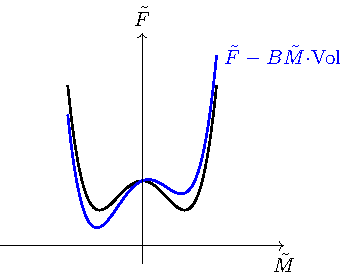
\includegraphics{figures/free_energy_in_external_field.pdf}
    \caption{free energy in external field}
\end{figure}
\begin{equation}
  \tilde{F} = \tilde{F} - B \tilde{M} \cdot \text{Vol}.
\end{equation}
and we have 
\begin{equation}
    \mathcal{Z}\left( B \right)  = \mathrm{e}^{- \frac{F\left( B \right)}{T}} = \int_{-\infty}^{\infty} \mathrm{d}\tilde{M} \, \mathrm{e}^{-\frac{1}{T} \left( \tilde{F} - B \tilde{M} \cdot \text{Vol} \right) } ,
\end{equation}
which is dominated by the double well in $\tilde{F}$.
Meanwhile, we have the relation
\begin{equation}
    M = \frac{1}{\text{Vol}} \frac{\partial F}{\partial B} = \frac{1}{\mathcal{Z}} \frac{\partial \mathcal{Z}}{\partial B} = \left< \tilde{M} \right> 
\end{equation}
and
\begin{equation}
  \chi = \frac{\partial M}{\partial B} = \frac{1}{\mathcal{Z}} \frac{\partial^2 \mathcal{Z}}{\partial B^2} - \frac{1}{\mathcal{Z}^{2}} \frac{\partial \mathcal{Z}}{\partial B} \frac{\partial \mathcal{Z}}{\partial B} = \left< M^{2} \right> - \left< M \right>^{2}
\end{equation}
% !TeX root = 场论与凝聚态.tex

\section{Adding Topology Structures to XY Model}
In classical statistic mechanics, XY model is widely proposed to describe the interactions between superconductors, whose weight reads
\begin{equation}
  \mathcal{Z} = \left( \prod_{\text{vertex}}^{} \int_{-\pi}^{\pi} \frac{\mathrm{d} \theta _{l}}{2\pi} \right) \prod_{\text{link}}^{} W \left( \mathrm{e}^{\mathrm{i} \mathrm{d} \theta_{l}} \right),
\end{equation}
where $W$ is the Boltzmann weight of the system, restricted by the $U(1)$ symmetry of $\theta$.
% !TeX root = 场论与凝聚态.tex

\section{Mixed Anomaly between $U(1)$ and $\tilde{U}(1)$}
In XY model, the expression of weight is
\begin{equation}
  \text{weight} = \frac{1}{T} \sum_{l} \left( \cos (\mathrm{d} \theta_{l}) -1\right).
\end{equation}
There exists a $U(1)$ global symmetry,
\begin{equation}
  \theta_{v} \to \theta_{v} + \alpha_{v},\quad \alpha \in U(1), \quad \mathrm{d} \alpha = 0 \mod 2\pi.
\end{equation}

We have known the order parameter of $U(1)$ global symmetry is $\mathrm{e}^{\mathrm{i}\theta_{v}}$, which \textbf{transforms with the global $U(1)$ symmetry transformation}.
We can construct invariant observables with order parameters, to determent the correlation scale or other properties of the system. Non-trivial observables should be $\left< \mathrm{e}^{\mathrm{i} \theta} \mathrm{e}^{- \mathrm{i}\theta_{v'}} \right>$ or more generally, 
\begin{equation}
  \left< \mathrm{e}^{ \mathrm{i} \sum_{v} B_v \theta _{v}} \right> =
  \begin{cases}
    0, & B_v \neq \nabla W_l \\
    $non zero$, & B_v = \nabla W \ ({}= \mathrm{d} ^{*} W)
  \end{cases}
\end{equation}
for the later case, we can obtain the following equation by lattice integration by part. If $B_v = \mathrm{d} ^{*} \left( W_l \right)$,
\begin{equation}
  \left< \mathrm{e}^{\mathrm{i}\sum_{v} B_v \theta_{v}} \right> = \left< \mathrm{e}^{\mathrm{i}\sum_{v} \left( \mathrm{d}^{*} \theta_{l} \right)W_l} \right>
\end{equation}
which is an invariant under $U(1)$.

\subsection{XY Model in $U(1)$ Background}
Coupling to a $U(1)$ background field, the weight of XY model becomes
\begin{equation}
  \text{weight} = \frac{1}{T} \sum_{l}  \left[ \cos \left( \mathrm{d} \theta_{l} - q A_l \right) -1 \right].
\end{equation}
In this case, $U(1)$ global symmetry manifests as $U(1)$ invariance, as we require $A_l$ transforms with $\theta_{v}$
\begin{equation}
  \begin{cases}
    \theta_{v} \to \theta_{v} + \alpha _{v}, & \alpha \in  U(1) \\
    A_l \to A_l + \mathrm{d} \alpha _{l}
  \end{cases}
\end{equation}
where now $\alpha _{v}$ is \emph{arbitrary}, without restriction of $\mathrm{d} \alpha _{l} = 0 \mod 2 \pi $.

Note that the transformation $A_{l} \to A_{l} + \mathrm{d} \alpha _{l}$ gives
\begin{equation}
  \mathcal{Z}[A] = \mathcal{Z}[A + \mathrm{d} \alpha],
\end{equation}
which means different backgrounds (with the difference of a total derivation) are equivalent.

This $A_l$ seems like a electromagnetic field, let us check its current behaviour. Take a Fourier transformation (or Poisson resummation), in current representation we get
\begin{equation}
  \prod{l} I_{j l} \left( \frac{1}{T} \right) \mathrm{e}^{\mathrm{i} j_{l} \left( \mathrm{d} \theta_{l} + q A_l \right)}
\end{equation}
we hope that $A_l$ should be $2 \pi $ periodic, thus $q$ must be a integer.\footnote{We can also couple the $\theta _{v}$ to a series of $A_l$'s, in this case, $\frac{q}{q'}$ must be a rational number.}

The operator correlation transforms as 
\begin{equation}
  \left< \mathrm{e}^{\mathrm{i} \theta_{v}} \mathrm{e}^{- \mathrm{i} \theta _{v'}} \right>_{A} = \mathrm{e}^{\mathrm{i} \left( \alpha _{v} - \alpha _{v'} \right) } \left< \mathrm{e}^{\mathrm{i} \theta _{v}} \mathrm{e}^{-\mathrm{i} \theta _{v'}} \right>_{A + \mathrm{d} \alpha}
\end{equation}

\subsection{Villain Model in $U(1)$ Background}
In Villain model, we have made the substitution,
\begin{equation}
  \cos (\mathrm{d} \theta) -1 \to \frac{1}{2} \mathrm{d} \theta^{2}
\end{equation}
thus it has no natural $2 \pi $ periodicity. We add this manually, by introducing a dynamical degree of freedom $m$ to be summed in path integral. The weight of Villain model is
\begin{equation}
  - \frac{1}{2T} \sum_{l} \bigl( \underbrace{\mathrm{d} \theta + 2 \pi m}_{\gamma _{l}} - A \bigr)_{l}^{2}.
\end{equation}
$m$ transforms with $\theta $ and $A_l$,
\begin{equation}
  \begin{cases}
    A_l \to A_l + \mathrm{d} \alpha _{l} + 2 \pi k_{l}, \\
    \theta_{v} \to \theta _{v} + \alpha _{l} + 2 \pi n_v, \\
    m_l \to m_l + k_l - \mathrm{d} n_l,
  \end{cases}
  \quad \alpha _{v} \in (-\pi ,\pi ],\ k_l, n_v \in \mathbb{Z}
\end{equation}
In this case, the vortex previous is no longer well-defined, as
\begin{equation}
  v_p \equiv \frac{\mathrm{d} \gamma _{p}}{2 \pi} = \mathrm{d} m_p \to \mathrm{d} m_p + \mathrm{d} k_p,
\end{equation}
$v_p$ isn't a invariant now.

We need to find a well-defined vortex. A simple choice would be
\begin{equation}
  \overline{v_p} \equiv \frac{\mathrm{d} \left( \gamma - A \right)}{2 pi},
\end{equation}
which is an invariant under gauge transformation,  but it is \emph{no longer an integer}.

Recalling that we have defined a vortex operator $V_p$ under the limit of $u \to+ \infty $, which is coupled with $\theta_{v}$ as 
\begin{equation}
  - \frac{u}{2} \sum_{p} \left( v_p - V_p \right)^{2} \xlongrightarrow[u \to +\infty]{\text{H-S trans.}} \mathrm{i} \sum_{p} \tilde{\theta}_{p} \left( v_p - V_p \right).
\end{equation}
This can be viewed as a Lagrangian constrain multiplier to restrict the vortex number equal to $V_p$.\footnote{Or get the same result by completing the integration getting a $\delta$ function.}
If we let $V_p \to V_p + \mathrm{d} k_p$, the theory is compatible with the transformation. However, $A_l$ and $V_p$ are no longer independent, i.e., they together form $U(1)$ background. The $U(1)$ field is described by
\begin{equation}
  \left( \mathrm{d} A - 2\pi V \right)_{p} \in \mathbb{R}.
\end{equation}
instead of the previous one $\mathrm{d} A_l \in U\left(1\right)$. This $\mathrm{d} A - 2\pi V$ can be regarded as a Villainized electromagnetic field, which indicates that \emph{a $2\pi $ flux cannot be distinguished with a vortex}.


\input{场论与凝聚态临时.tex}


\end{document}
